\subsection{Asistente personal y módulo de progreso}\label{sec:asistente}

Además del plan, el MVP incluye un \textbf{asistente personal} en forma de chat y una sección de \textbf{progreso}. La sección de recomendaciones dejó de ser una lista de textos: ahora son tarjetas por categoría (foco, riesgo, estrategia, carga, bienestar, estudio y progreso) y, al tocar una, el chat la explica con pasos, fechas del plan del estudiante, gráficas sencillas y la evidencia que la respalda; luego la persona puede preguntar.

\textbf{Flujo de una consulta.} (1) El mensaje se normaliza (minúsculas, sin tildes). (2) Se detecta la intención por coincidencia de raíces de palabras, con puntaje; si una pregunta mezcla un método de estudio con una intención de horario, gana el método salvo que se pregunte por hoy, mañana o ahora. (3) Un manejador consulta el plan, las tareas y las estadísticas y arma la respuesta como una lista de \emph{bloques} tipados (párrafo, lista, línea de tiempo, barras con línea de límite, ciclo de enfoque y pausa, plantilla copiable y evidencia) que la interfaz dibuja. (4) Se ofrecen preguntas sugeridas. Si ninguna intención aplica y hay un modelo local disponible, la pregunta pasa a la capa opcional descrita en la sección~\ref{sec:tipo-ia}.

\textbf{Qué responde.} Preguntas sobre el horario (qué hay hoy o mañana, qué sigue, próximas entregas, si va atrasado, cuándo está libre, créditos y horas de estudio, calibración y progreso), cómo prepararse para un parcial y métodos de estudio y bienestar. También hace una \textbf{entrevista de cinco preguntas} (mejor momento del día, cómo estudia, qué lo distrae, cuántas horas duerme y su mayor reto) con la que arma un \textbf{plan de estudio personal}: unas reglas eligen los métodos que corresponden al perfil y los ubican en los huecos de su plan (figura~\ref{fig:perfil}).

\textbf{Base de métodos.} El asistente solo recomienda métodos incluidos en una base propia de doce temas, cada uno con qué es, por qué funciona, pasos y referencias (tabla~\ref{tab:metodos}). Cuando una convención no tiene sustento científico, el texto lo dice (por ejemplo, que los 25 minutos de la técnica Pomodoro son una costumbre útil y no una regla científica).

\begin{table}[H]
\centering\small
\caption{Métodos de estudio y bienestar de la base del asistente}\label{tab:metodos}
\begin{tabularx}{\textwidth}{>{\raggedright\arraybackslash}p{4.6cm} >{\raggedright\arraybackslash}X >{\raggedright\arraybackslash}p{3.6cm}}
\toprule
Método & Idea central & Evidencia \\
\midrule
Práctica de recuperación & Recordar sin mirar en lugar de releer & \cite{Roediger2006,Dunlosky2013} \\
Repetición espaciada & Repartir los repasos en varios días & \cite{Cepeda2006,Dunlosky2013} \\
Práctica intercalada & Mezclar tipos de problema en una sesión & \cite{Rohrer2007,Dunlosky2013} \\
Autoexplicación & Explicar el tema con palabras propias & \cite{Chi1994,Dunlosky2013} \\
Bloques de enfoque con pausas & Pausas breves para sostener la atención & \cite{Ariga2011} \\
Planes «si\dots entonces\dots» & Definir de antemano cuándo y dónde empezar & \cite{Gollwitzer2006} \\
Cómo arrancar cuando se posterga & Reducir el costo de empezar & \cite{Steel2007} \\
Dormir como parte del estudio & Proteger el sueño antes de una prueba & \cite{Curcio2006} \\
Movimiento y pausas activas & Actividad física regular & \cite{Hillman2008} \\
Celular fuera de la vista & Reducir distracciones durante el bloque & \cite{Ward2017} \\
Manejar los nervios & Escribir las preocupaciones antes de la prueba & \cite{Ramirez2011} \\
Qué evitar: releer y subrayar & Técnicas de baja utilidad & \cite{Dunlosky2013} \\
\bottomrule
\end{tabularx}
\end{table}

Estos estudios describen efectos promedio en poblaciones concretas; el asistente los presenta como orientación y no como garantía de un resultado individual, y ante nervios intensos recomienda buscar apoyo profesional.

\textbf{Progreso.} La sección de progreso se alimenta de lo que el estudiante registra: bloques marcados como cumplidos, las horas reales que anota al terminar un trabajo y los días en que abre la aplicación. Para cada semana calcula tres cantidades: las horas \emph{necesarias}, que salen de los créditos ($\sum_{m}\max(0,\,3c_m-h_{clase,m})$ sobre las materias $m$); las horas \emph{planeadas}, que son las que el plan le propone; y las horas \emph{cumplidas}, que son las registradas. Con ellas se muestran el porcentaje de la meta, un gráfico de las últimas ocho semanas, el avance por materia, las tareas terminadas por semana, un mapa de actividad de 35 días y dos rachas: de estudio (días seguidos con horas registradas) y de uso. La racha actual no se rompe si hoy todavía no hay actividad, para no castigar al estudiante a mitad del día. Las figuras~\ref{fig:progreso} y~\ref{fig:asistente} muestran ambas pantallas con datos de ejemplo.

\begin{figure}[H]
\centering
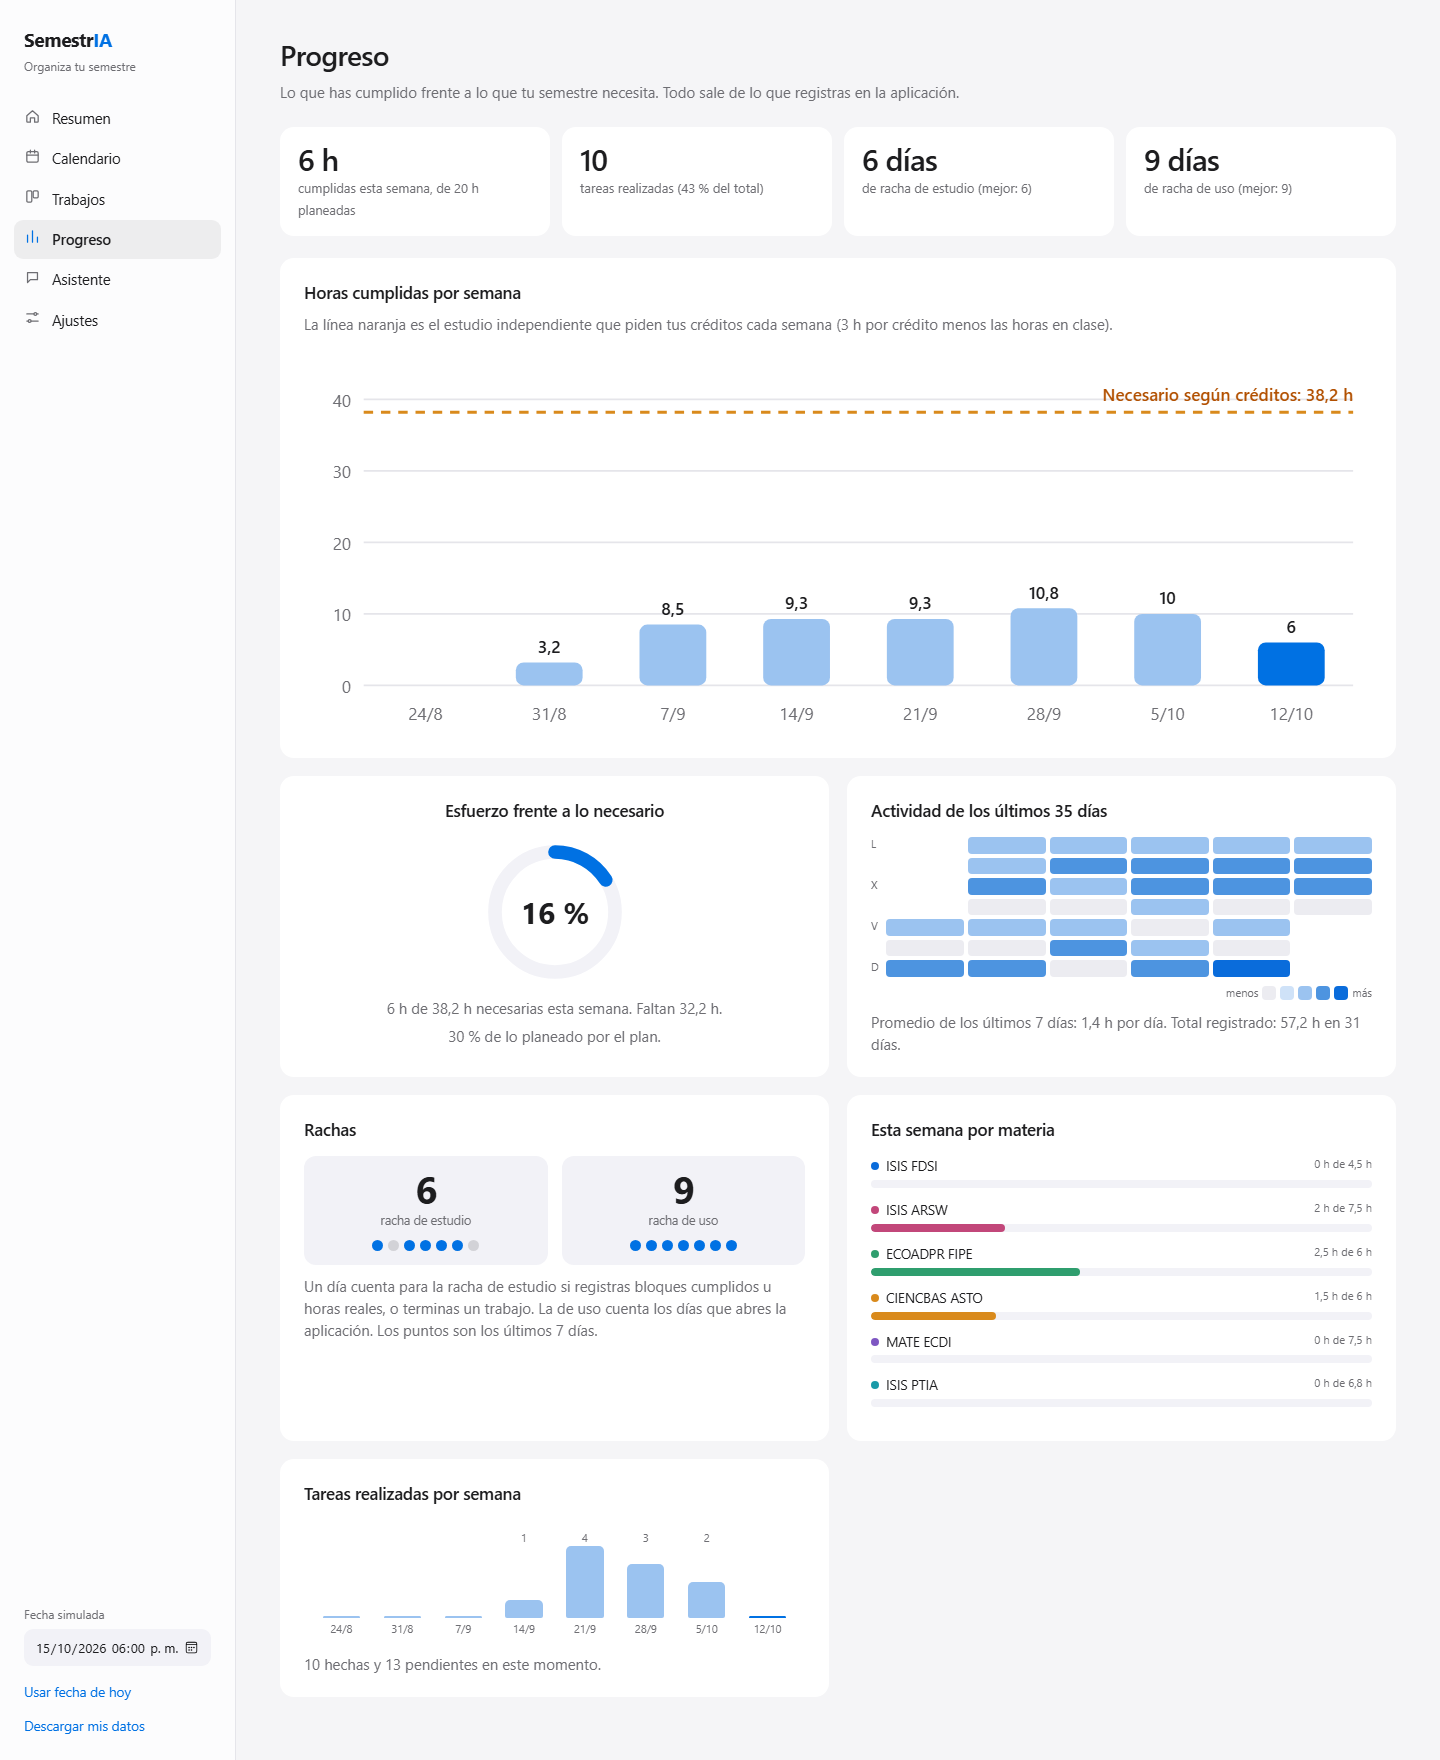
\includegraphics[width=\textwidth]{img/pant_09_progreso.png}
\caption{Progreso: horas cumplidas frente a las necesarias, tareas realizadas, mapa de actividad y rachas (datos de demostración)}\label{fig:progreso}
\end{figure}

\begin{figure}[H]
\centering
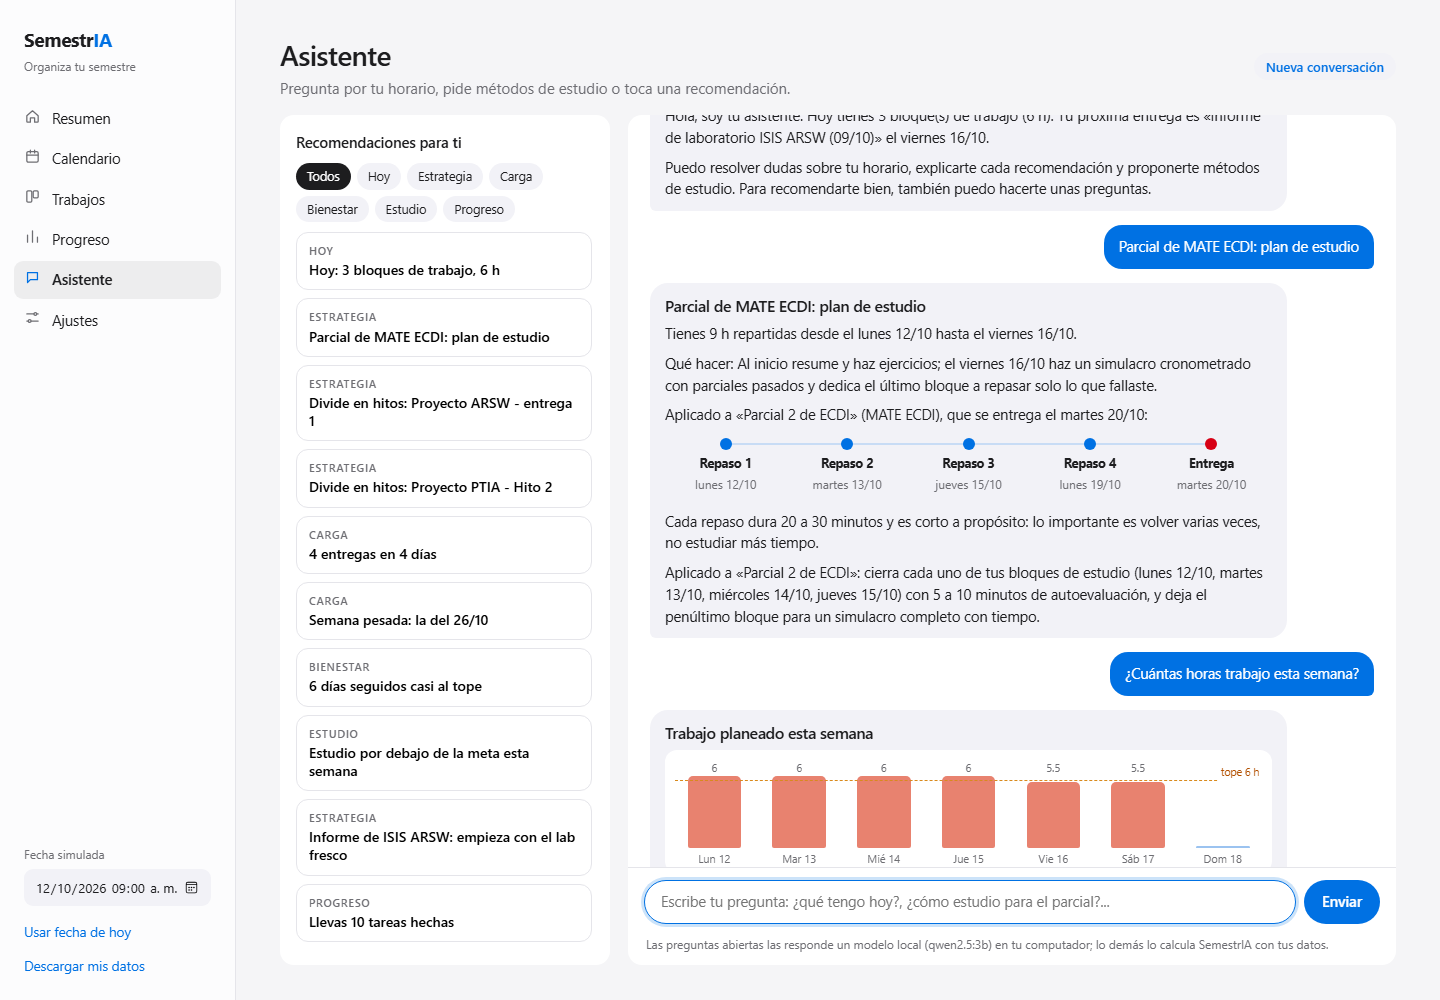
\includegraphics[width=\textwidth]{img/pant_10_asistente.png}
\caption{Asistente personal: recomendaciones por categoría y chat que las explica (datos de demostración)}\label{fig:asistente}
\end{figure}

\begin{figure}[H]
\centering
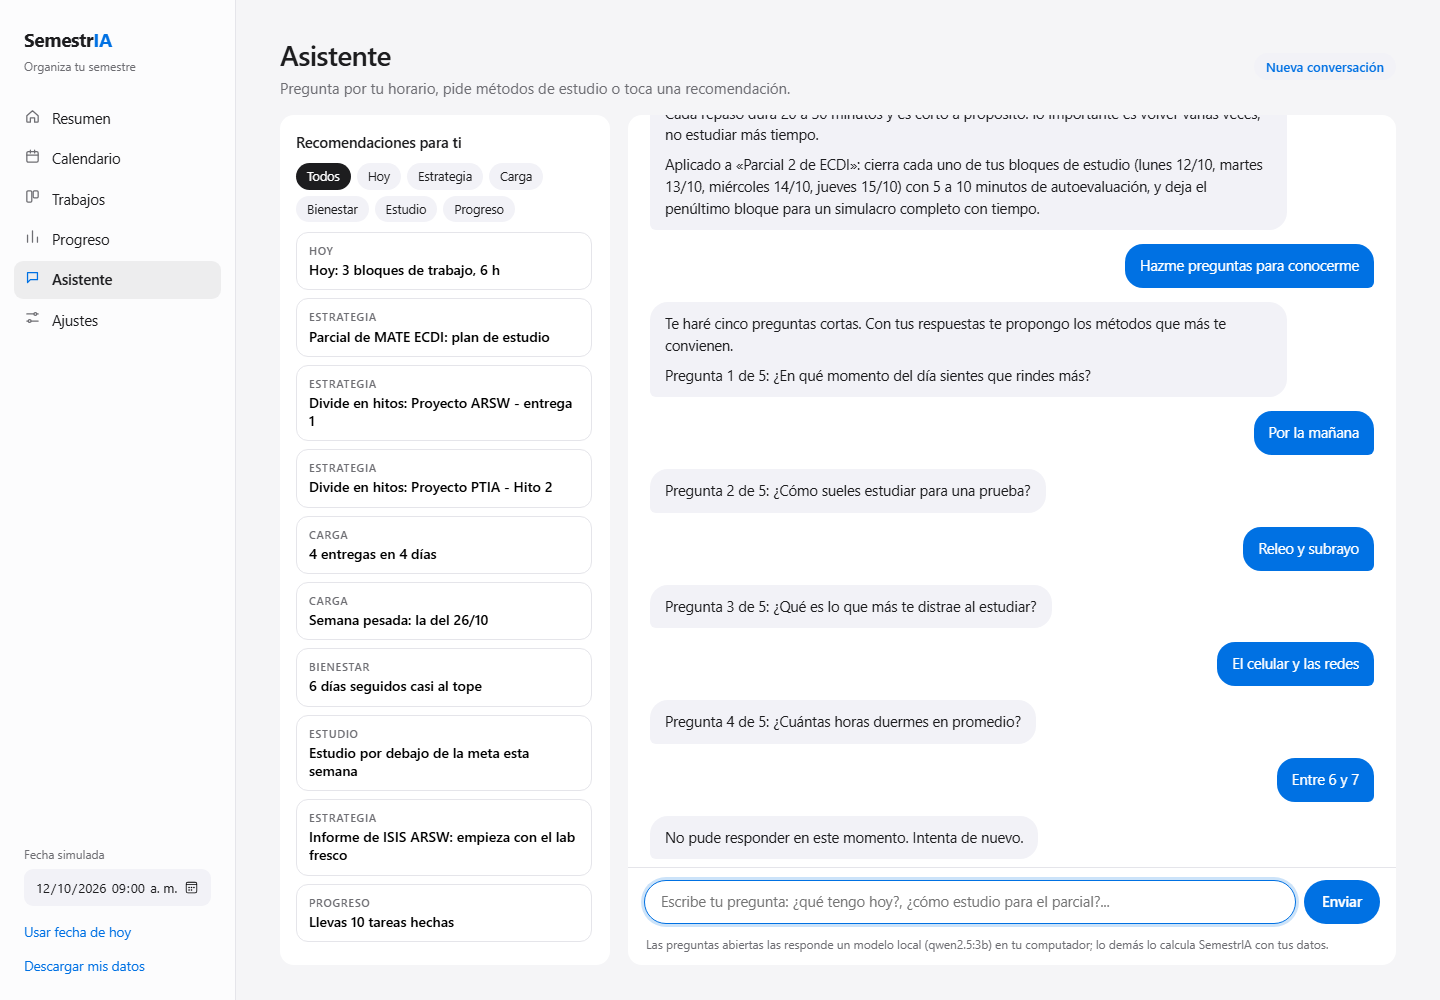
\includegraphics[width=\textwidth]{img/pant_11_asistente_perfil.png}
\caption{Entrevista de cinco preguntas y plan de estudio personal}\label{fig:perfil}
\end{figure}
